\documentclass[runningheads,a4paper]{llncs}

\usepackage{amssymb}
\setcounter{tocdepth}{3}
\usepackage{graphicx}
\usepackage{url}
\usepackage{floatrow}
\newcommand{\keywords}[1]{\par\addvspace\baselineskip
\noindent\keywordname\enspace\ignorespaces#1}

\pagestyle{headings}

\begin{document}

\mainmatter  % start of an individual contribution

% first the title is needed
\title{Choosers: designing a highly expressive algorithmic music composition system for non-programmers}

% a short form should be given in case it is too long for the running head
\titlerunning{Choosers: algorithmic music composition system for non-programmers}

% the name(s) of the author(s) follow(s) next
%
% NB: Chinese authors should write their first names(s) in front of
% their surnames. This ensures that the names appear correctly in
% the running heads and the author index.
%
\author{Matt Bellingham\inst{1}, Simon Holland\inst{2} and Paul Mulholland\inst{2}}
%
% if the names of the authors are too long for the running head, please use the format: AuthorA et al.
\authorrunning{Bellingham, Holland and Mulholland}

% the affiliations are given next; don't give your e-mail address
% unless you accept that it will be published
\institute{University of Wolverhampton \and The Open University\\ \email{matt.bellingham@wlv.ac.uk}}

%
% NB: a more complex sample for affiliations and the mapping to the
% corresponding authors can be found in the file "llncs.dem"
% (search for the string "\mainmatter" where a contribution starts).
% "llncs.dem" accompanies the document class "llncs.cls".
%


\maketitle


\begin{abstract}

We present an algorithmic composition system designed to be accessible to those with minimal programming skills and little musical training, while at the same time allowing the manipulation of detailed musical structures more rapidly and more fluidly than would normally be possible for such a user group. These requirements led us to devise non-standard programming abstractions as the basis for a novel graphical music programming language in which a single basic element permits indeterminism, parallelism, choice, multi-choice, recursion, weighting and looping. The system has general musical expressivity, but for simplicity here we focus on manipulating samples. The musical abstractions behind the system have been implemented as a set of SuperCollider classes to enable end-user testing of the graphical programming language via a Wizard of Oz prototyping methodology. The system is currently being tested with undergraduate Music Technology students who are typically neither programmers, nor traditional musicians.


\keywords{music, composition, algorithmic composition, graphical programming, music programming languages, interaction design, user interface}

\end{abstract}


\section{Introduction}\label{introduction}

Algorithmic composition systems are able to support creativity in a number of ways \cite{jacob} but these tools are generally only available to programmers. We present an algorithmic composition system designed to be accessible to users without programming skills and with minimal musical training. The intention is to enable the manipulation of detailed musical structures more rapidly and more fluidly than would normally be possible for such a user group.

These requirements led us to iteratively develop, via the programming walkthrough method \cite{bell}, non-standard programming abstractions such as the chooser (see Fig.~\ref{fig:annotated-chooser}) which in a single basic element enables indeterminism, parallelism, choice, multi-choice, recursion, weighting, and looping. The system has general musical expressivity, but for simplicity here we focus on manipulating samples.

The system is designed with the following principles in mind:

\begin{itemize}
	\item
	Parsimony -- a small number of consistent powerful ideas do the work combinatorially;
	\item
	Musically meaningful structuring actions are simple and quick to do;
	\item
	Both bottom-up and top-down construction are allowed in any combination;
	\item
	Affordances are designed for users of varying music computing abilities via progressive disclosure.
\end{itemize}

The musical abstractions behind the system have been implemented as a set of SuperCollider \cite{supercollider} classes to enable end-user testing of the graphical programming language during development via a Wizard of Oz prototyping methodology. The system is being tested with undergraduate Music Technology students who are typically neither programmers nor traditional musicians. While they may be conversant with some elements of music theory, their background is often as self-taught music producers with experience of making music electronically using music sequencers/DAWs.

In order to illustrate the principles behind the system, we will present its principal elements in turn, starting from the most elementary.


\section{The play area and playing samples}\label{play-area}

The largest central area of the user interface is known as the play area. It is here that the user is able to assemble, audition, and package musical structures. For someone who wishes to work bottom-up (i.e. starting from existing samples), the simplest way to start is to drag samples into the play area. Samples are shown in boxes (see Fig.~\ref{fig:samples}) and can be auditioned by clicking on the box.


\begin{figure}
	\begin{floatrow}
		\ffigbox{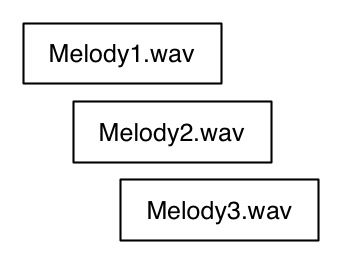
\includegraphics[height=3cm]{images/samples.png}}
			{\caption{Samples dragged into the play area.}\label{fig:samples}}
		\ffigbox{	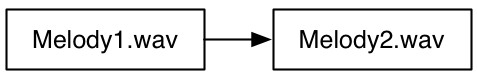
\includegraphics[height=0.8cm]{images/simple-sequence.png}}
			{\caption{An example of a simple sequence.}\label{fig:simple-sequence}}
	\end{floatrow}
\end{figure}


Samples, shown in boxes in the play area, can be assembled into a sequence. A sequence is shown by arrows connecting boxes (see Fig.~\ref{fig:simple-sequence}). The direction of the arrow indicates the order of the sequence. Once the first sample has finished playing the second sample will begin. Only a single arrow can enter or exit each element in a sequence. Boxes and sequences can be put inside other boxes, thereby packaging them into a single unit. Anything in a box can be played by clicking on it.
 
So far, nothing is remotely novel.  However, in Section~\ref{choosers} we turn to powerful abstractions called choosers. These have a less familiar set of affordances and are the principal source of power of the new formalism.



\section{Soundable choosers}\label{choosers}

Boxes referring to samples or sequences can be snapped together vertically to create what are known as soundable choosers. Soundable choosers combine indeterminism, choice, parallelism, multi-select weights, looping, and abstraction in a single language element, as explained in detail below.

\begin{figure}
	\begin{floatrow}
		\ffigbox{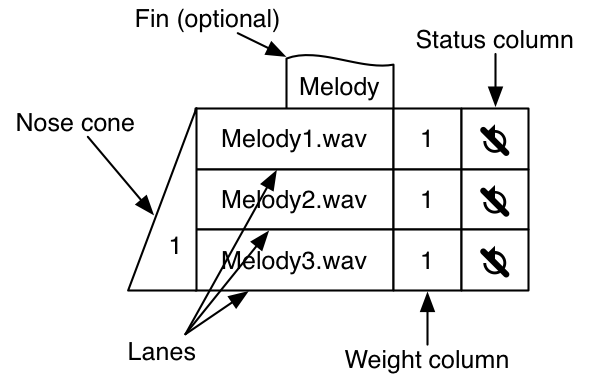
\includegraphics[height=4cm]{images/annotated-chooser.png}}
	{\caption{A soundable chooser showing each
		element.}\label{fig:annotated-chooser}}
		\ffigbox{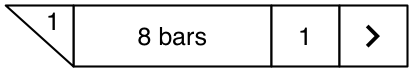
\includegraphics[height=0.8cm]{images/time-chooser.png}}
	{\caption{A time chooser with a duration of 8
		bars.}\label{fig:time-chooser}}
	\end{floatrow}
\end{figure}


Each box in a soundable chooser has its own lane. If there are two or more lanes in a chooser, the lane will display three additional elements: the nose cone on the left, and the weight column and status column on the right. The nose cone allows the user to specify how many of the lanes will be played simultaneously. For example, if there are fives lanes, and the nose cone contains the number two, two lanes will be chosen to play simultaneously.  If the nose cone contains the number one, only a single lane will be chosen. Note that every time the chooser is played, the choice of lanes is made afresh non-deterministically (i.e. at random).
 
The weight column, shown immediately to the right of the sample name, determines the relative likelihood of a lane to be selected for playback. Fig.~\ref{fig:annotated-chooser} shows three lanes each with a weight of one, meaning they are equally likely to be selected. If one lane's weight was changed to two it would now be more likely to be selected for playback. If a lane is given a weight of zero it will never be selected for playback. This can be a useful way of trying arrangement ideas without removing the lane altogether. The status column shown on the far right of each lane allows for control over how the chooser deals with looping and stopping playback, as we will describe in detail below. 
 
Just as samples can be assembled into sequences, so can soundable choosers. The nose cone can be set to zero, which will result in the soundable chooser being skipped in the context of a sequence. Optionally, the fin can be used to give the chooser a name, such as the chooser named `Melody' in Fig.~\ref{fig:annotated-chooser}.




\section{Time lanes and time choosers}\label{time-lanes-and-time-choosers}

A time lane is a lane whose purpose is to specify a musical duration (usually in beats or bars or seconds) rather than to specify something to be sounded. 
 
A time lane can be included in what is known as a time chooser (see Fig.~\ref{fig:time-chooser}). Note that the time chooser has a nose cone which contrasts visually with the nosecone of a soundable chooser. Time choosers and soundable choosers have similarities and differences. They are similar in that both make nondeterministic selections from the lanes they contain. However the business of a soundable chooser is to choose one or more lanes to be sounded, whereas the business of a time chooser is to choose a single duration. A time chooser can select only a single time lane or none -- depending on the number in its nose cone. It is impossible for a time chooser to select multiple durations at once.
 
A time chooser can be used alone as part of a sequence -- however, when used in this way it will simply result in a rest of the specified duration. A time chooser has more interesting behavior when combined with a soundable chooser, as detailed below.

A soundable chooser can be given a limited musical duration by adding a time chooser to its bottom (see Fig.~\ref{fig:full-chooser}) - note how the nose cones fit together. The duration of the soundable chooser will now be controlled by the time chooser. Together the two types of chooser are referred to as a full chooser, or just a chooser for short.

The purpose of a time chooser within a full chooser is to moderate in a non-deterministic manner how long the soundable chooser and its individual lanes play. Possible interactions between the settings of soundable and time choosers can make the results more varied than might be imagined, as demonstrated in the following example.


\begin{figure}
	\begin{floatrow}
		\ffigbox{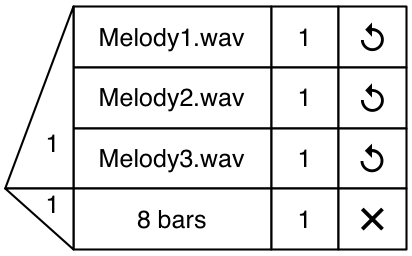
\includegraphics[height=3cm]{images/full-chooser.png}}
	{\caption{A full chooser, consisting of a soundable chooser and a time chooser.}\label{fig:full-chooser}}
		\ffigbox{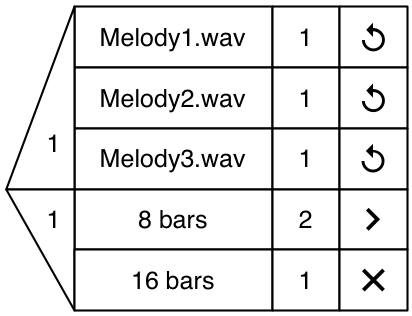
\includegraphics[height=3.5cm]{images/two-time-choosers.png}}
	{\caption{A chooser with two lanes in the time chooser. Only one will be selected. Note the different weights which make an 8 bar duration more likely, the soft stop for the 8 bar option, and the hard stop for the 16 bar option.}\label{fig:two-time-choosers}}
	\end{floatrow}
\end{figure}


Fig.~\ref{fig:full-chooser} shows a full chooser consisting of a soundable chooser containing three samples, and a time chooser with a duration of eight bars. The status column of the time chooser shows either a soft stop (shown as \textgreater) or a hard stop (shown as $\times$). In this example, one of three samples will be selected for playback. All samples are set to loop, as shown by the circular arrow. When the duration shown in the time chooser (8 bars) has elapsed the currently-playing sample will be stopped. As the sole lane of the time chooser is set to a hard stop, the sample selected by the soundable chooser will be stopped as soon as time is up. If, by contrast, it were set to a soft stop, the sample would not be stopped at this point -- instead the loop controlling the sample would be turned off and the sample would play to its end. Consequently, if the sample was shorter than 8 bars duration, it would loop one or more times before playing to its end after the loop was switched off. If the sample were longer than 8 bars, the entire sample should play just once.
 
In general, a time chooser's nose cone can be set to either one or zero. If it is set to zero the soundable chooser will run as though there is no time chooser. This allows for quick arrangement changes, with the possibility of infinite playback if the soundable chooser lanes are set to loop. If the soundable chooser is not set to loop the sample(s) will play and the chooser will be released when they have finished playing, regardless of length.
There can be more than one time lane in a chooser (see Fig.~\ref{fig:two-time-choosers}), but only one will be selected when the chooser runs. The selection is made using the same lane weight system as for soundable lanes.

Sometimes it is desirable to ensure that a chooser lane is always selected for playback. Any soundable lane with `A' in the weight column will always be selected and played. The number in the soundable chooser nose cone is constrained by these mandatory lanes; for example, in the example shown in Fig.~\ref{fig:always} the soundable chooser nose cone number can only be three (play all) or zero (do not play any lanes: this can result in a rest if the time chooser selects a duration, or skipped if both soundable and time choosers have nose cone values of zero).


\begin{figure}
	\begin{floatrow}
		\ffigbox{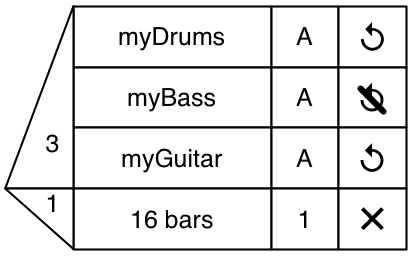
\includegraphics[height=3cm]{images/always.png}}
	{\caption{A chooser with three lanes set to always play.}\label{fig:always}}
		\ffigbox{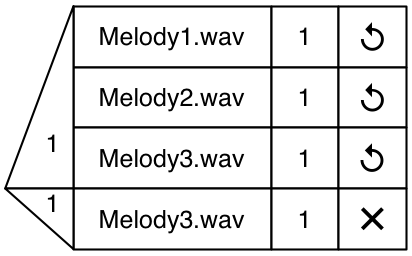
\includegraphics[height=3cm]{images/sample-time.png}}
	{\caption{The duration of the \texttt{melody3.wav} sample is used in the
		time chooser. Note that \texttt{melody3.wav} is also one of the samples
		in the soundable chooser and so it is used for both duration and
		playback.}\label{fig:sample-time}}
	\end{floatrow}
\end{figure}




\section{Setting the duration using the length of a
	sample}\label{setting-the-duration-using-the-length-of-a-sample}

Although the duration in a clock lane is usually specified by a number of beats, bars, or seconds, it can also be specified by a sample. It is important to note that any sample added to a time chooser will not be audible; instead its duration is used to control the time. In order for a sample to be both audible and used to set the duration of the chooser,  it is necessary to add it to both the soundable and time choosers. An example is shown in Fig.~\ref{fig:sample-time}.




\section{Boxes and repetition}\label{sec:sequence}

% Since boxes can always be put into sequences, it follows that we can also construct sequences of any mixture of playables.

% As previously noted, sequences are shown by arrows (see Fig.~\ref{fig:simple-sequence}). The direction of the arrow denotes the next item in the sequence.  There is ony ever zero or one immediately next items in a sequence, since if we want  parallelism or choices, we can always use a chooser. Once the first playable has finished playing the second playable will begin.
Boxes can contain any playable (samples, choosers or sequences) or refer to them by name. Note that the example in Fig~\ref{fig:repetition} uses boxes which refer to playables named `Joe Verse' and `Joe Chorus'. The system allows the use of such references even when a playable of that name does not yet exist; this allows the user to create placeholders without having to immediately populate them. Importantly, this allows users to work using either a top-down or bottom-up approach. A top-down approach is when the user begins with a high-level outline of the piece (an ABA structure, for example) and then populates those sections, working down to the note or sample level. A bottom-up approach is the opposite: the user begins at the note or sample level and builds musical sections before organising the macro structure of the piece. 
% More technically, it is generally possible to play an incompletely specified sequence up to the point where a reference is not understood.


Explicit repeats can be added via multiplication notation below playables or references to playables, as shown in Fig.~\ref{fig:repetition} and Fig.~\ref{fig:repetition-durations}.

\begin{figure}
	\centering
	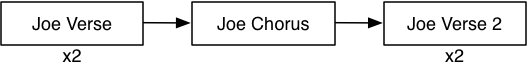
\includegraphics[height=1cm]{images/repetition.png}
	\caption{A simple sequence showing the use of repetition notation.}\label{fig:repetition}
\end{figure}

% removed: Note that if a soundable chooser without a timing master is repeated in this way all lane loops are defeated


\begin{figure}
	\centering
	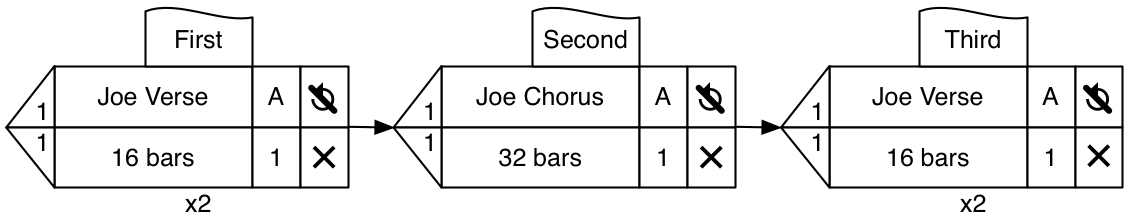
\includegraphics[height=2.3cm]{images/repetition-durations.png}
	\caption{The same sequence as shown in Fig~\ref{fig:repetition} but with the duration of each repetition constrained using a time chooser.}\label{fig:repetition-durations}
\end{figure}



\section{Nesting and recursion}\label{nesting-and-recursion}

So far, musical structures have been assembled largely bottom-up via sequencing, looping, choice and multi-choice (possibly weighted), non-determinism and packaging. In this section we see how high level structures can be elaborated downwards using nesting and recursion.
 
The first column of any lane is actually a box, and consequently can make reference to any other chooser or element. Thus, one chooser can be nested inside another chooser, either visually or by referencing a named chooser. In the example shown in Fig.~\ref{fig:nesting}, due to the number three in the nose cone, the parent soundable chooser will always select all three lanes. The top two lanes contain child soundable choosers which will select one of two samples. The \texttt{Drums.wav} sample will always play. The duration of the full chooser is controlled by the time chooser which is set to hard stop after a duration of 32 bars. Importantly, in terms of understanding the effect of time constraints on nested choosers, note that in this example the child choosers are not set to loop, while the parent lanes are set to loop. Thus, if the chosen child sample has a duration under 32 bars, the parent lane will loop and re-select a sample until the time chooser's duration expires and playback is stopped.


%\begin{figure}[!h]
%	\begin{floatrow}
%		\ffigbox{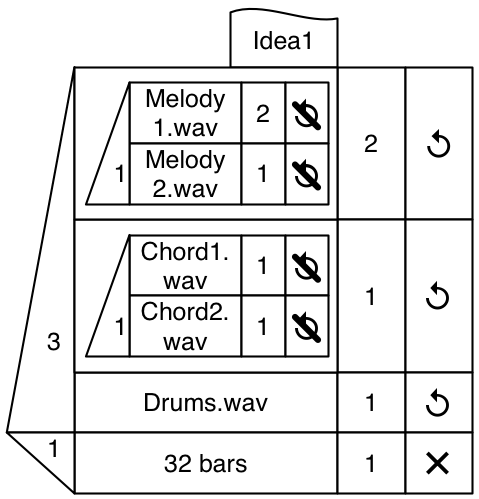
\includegraphics[height=4.1cm]{images/nesting.png}}
%	{\caption{An example of nesting, showing two soundable choosers nested
%		inside a parent chooser.}\label{fig:nesting}}
%		\ffigbox{\includegraphics[height=2.2cm]{images/variable.png}}
%	{\caption{An example of a variable named `Var'.}\label{fig:variable}}
%	\end{floatrow}
%\end{figure}

\begin{figure}
	\centering
	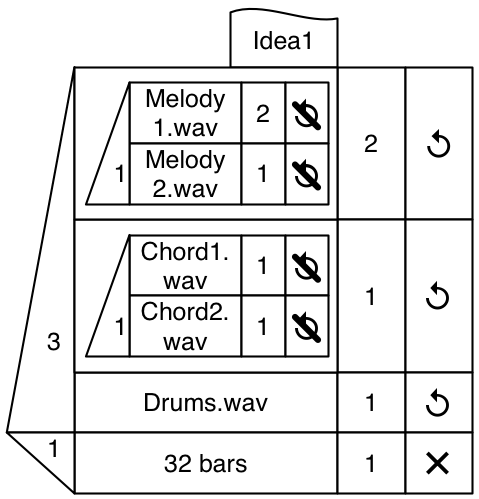
\includegraphics[height=4.8cm]{images/nesting.png}
	\caption{An example showing two soundable choosers nested
				inside a parent chooser.}\label{fig:nesting}
\end{figure}

An alternative to visually nesting a chooser is to simply reference a chooser's name (as given in the fin of the nested chooser) inside a lane of the parent chooser. This notation can be preferable to visual nesting in some situations as it allows for the reuse of musical material, as well as minimizing visual complexity. The user is free to use either notation in any combination.

This paper outlines core functionality but, due to space constraints, omits the mechanisms used to create, reuse, and coordinate variables and variable choices. Variables allow the user to easily reuse material (which can be integers, status types, or duration information) by defining a variable once and creating multiple references from that variable to a single element.


%\section{Variables and abstraction}\label{variables-and-abstraction}

% The abstractions so far give expressivity for constructing musical structures (though in this paper we omit the mechanism for mixing and effects). However, with the next step, the system is given Turing completeness.
 
%Variables allow the user to easily reuse material by defining a variable once and creating multiple references from that variable to a single element. Variables are not audible. Variables can contain integers, status types and duration information. A rounded nose cone makes them visually distinct from choosers. They are named via the fin, and do not require a status column. See Fig~\ref{fig:variable} for an example. In this paper we omit the mechanisms used to reuse previous variable values (used to control indeterminacy) and to coordinate variable choices.

% The guiding principle of indeterminacy means that, by default, variable bindings are re-run every time they are referenced. However, it is sometimes musically useful to  reuse previous values of variables. Consequently, the user is able to reuse previous values of variables by issuing a number or name after the variable name when it is referenced. In this way indeterminacy can be controlled. The format for this is `Name@ID', with the name being the name of the variable (in this case, `Var') and the ID being the number or name given by the user. Examples could be Var@2 or Var@verse.
 
% The user may want to coordinate variable choices; for example, if the chooser selects a duration of 16 bars it may also be wished to set the status to hard stop and set the previous chooser to repeat twice. This can be achieved by using a multi-column variable chooser as seen in Fig.~\ref{fig:multi-column-variable-1}. Note that the variable has multiple named columns. The required notation is `name:column'.


%\begin{figure}[!h]
%	\begin{floatrow}
%		\ffigbox{\includegraphics[height=5cm]{images/multi-column-variable-1.png}}
%	{\caption{A multi-column variable chooser, showing the name:column
%		referencing notation.}\label{fig:multi-column-variable-1}}
%		\ffigbox{\includegraphics[height=5cm]{images/multi-column-variable-2.png}}
%	{\caption{Coordinated multi-column variable chooser showing the use of
%		the Name@ID:column notation.}\label{fig:multi-column-variable-2}}
%	\end{floatrow}
%\end{figure}


%As with single-column variables, it is possible to append a number or name (the ID) to the variable when it is used in order to access the variable history and reuse a selection multiple times. The format for this is `name@ID:column'. Importantly, this allows for coordination between the columns of the variable chooser. 

%Fig.~\ref{fig:multi-column-variable-2} shows the use of an ID to reuse a variable selection.



% \section{Testing}


\section{Related work}

In a previous paper \cite{Bellingham} we have used the Cognitive Dimensions of Notations framework \cite{Green} to review the usability of a representative selection of software capable of algorithmic music composition. We found that most existing software requires the user to have a considerable understanding of constructs in either graphical (e.g Max, Pure Data) or text-oriented (e.g. SuperCollider, ChucK, Csound) programming languages: such knowledge requires a significant learning overhead. Users are often required to have an understanding of musical notation and/or music production equipment such as mixing desks and patchbays. Several pieces of software imposed working practices which were not conducive to compositional processes. In some instances the user was unable to define, and subsequently change, the musical structure. Finally, complex visual design in graphical programming languages led to patches with multiple connections, making them difficult to read and to navigate. 



\section{Conclusions}\label{emergent-design-principles}

This paper outlines a new abstraction, the chooser. The chooser system is designed to meet several needs: to enable our target users to create algorithmic music of arbitrary complexity; to facilitate graphical programming with minimal syntactical concerns; and to make common musical tasks simple. 

The work presented in this paper is based on a desire to create simplicity in a user interface for algorithmic music, and to offer consistency and flexibility with an emphasis on enabling musically useful structural changes to be made quickly and easily. While there are a number of programs capable of algorithmic music there is a lack of software designed for non-programmers. It is hoped that the design outlined here will enrich the tools available to composers and musicians.


\begin{thebibliography}{4}

\bibitem{jacob} Jacob, B. L.: Algorithmic Composition as a model of creativity, Organised Sound, Cambridge University Press, 1(03), pp. 157 -- 165. (1996)

\bibitem{bell} Bell, B., Citrin, W. V., Lewis, C., and Rieman, J.: The Programming Walkthrough: A Structured Method for Assessing the Writability of Programming Languages; CU-CS-577-92. Computer Science Technical Reports, Paper 554. (1992)

\bibitem{supercollider} McCartney, J.: Rethinking the Computer Music Language: SuperCollider. Computer Music Journal, 26(4) pp. 61 -- 68. (2002)

\bibitem{Bellingham} Bellingham, M., Holland, S., and Mulholland, P.: A Cognitive Dimensions analysis of interaction design for algorithmic composition software. In du Boulay, B. and Good, J., editors, Proceedings of Psychology of Programming Interest Group Annual Conference 2014, pp.  135 -- 140. (2014)

\bibitem{Green} Green, T. R. and Petre, M.:  Usability Analysis of Visual Programming Environments: a `cognitive dimensions' framework. Journal of Visual Languages and Computing, 7: pp. 131 -- 174. (1996)

\end{thebibliography}

\end{document}